\documentclass[a4]{article}

\usepackage[left=2cm,right=2cm,top=2cm,bottom=2cm]{geometry} 

\usepackage[utf8]{inputenc}   % otra alternativa para los caracteres acentuados y la "ñ"
\usepackage[           spanish % para poder usar el español
                      ,es-tabla % para los captions de las tablas
                       ]{babel}   
\decimalpoint %para usar el punto decimal en vez de coma para los números con decimales

%\usepackage{beton}
%\usepackage[T1]{fontenc}

\usepackage{parskip}
\usepackage{xcolor}

\usepackage{caption}

\usepackage{enumerate} % paquete para poder personalizar fácilmente la apariencia de las listas enumerativas

\usepackage{graphicx} % figuras
\usepackage{subfigure} % subfiguras

\usepackage{amsfonts}
\usepackage{amsmath}
\usepackage{listings}
\lstset{language=Python}          % Set your language (you can change the language for each code-block optionally)

\definecolor{gris}{RGB}{220,220,220}
	
\usepackage{float} % para controlar la situación de los entornos flotantes

\restylefloat{figure}
\restylefloat{table} 
\setlength{\parindent}{0mm}


\usepackage[bookmarks=true,
            bookmarksnumbered=false, % true means bookmarks in 
                                     % left window are numbered
            bookmarksopen=false,     % true means only level 1
                                     % are displayed.
            colorlinks=true,
            allcolors=blue,
            urlcolor=cyan]{hyperref}
\definecolor{webblue}{rgb}{0, 0, 0.5}  % less intense blue


\title{\Huge Inteligencia de Negocio. Práctica 1:\\
Resolución de problemas de\\
clasificación y análisis experimental \vspace{5mm}}

\author{\LARGE Patricia Córdoba Hidalgo \vspace{2mm}\\
  \Large patriciacorhid@correo.ugr.es \vspace{2mm}\\
  \Large Grupo 2 (Viernes) \vspace{5mm}}

\date{\today}

\begin{document}

\maketitle

\newpage
\tableofcontents
\newpage

\section{Introducción}

El objetivo de la práctica es clasificar los tumores encontrados en mamografías de distintos pacientes. Estos tumores pueden pertenecer a una de las siguientes clases: benignos o malignos. Estamos ante un problema de aprendizaje supervisado, más concretamente de clasificación.

Contamos con 961 instancias de datos de pacientes. Estos datos poseen los siguientes atributos:
\begin{itemize}
\item Código BI-RADS (nominal): Sistema de control de calidad. Un médico radiólogo asigna a la mamografía una categoría numérica después de interpretarla, con el objetivo de que el reporte radiográfico pueda ser entendido por múltuples médicos o centros hospitalarios.

\item Edad del paciente (entero).

\item Forma de la masa anormal detectada (nominal), pudiendo ser:\\
  \vspace{-5mm}
  
  R: Redonda.\\
  O: Ovalada.\\
  L: Lobular.\\
  I: Irregular.\\
  N: No definida.\\

   \vspace{-5mm}
\item Margen de masa (nominal):\\
  \vspace{-5mm}

  1: circumscribed.\\
  2: microlobulated.\\
  3: obscured.\\
  4: ill-defined.\\
  5: speculated.\\

   \vspace{-5mm}
\item Densidad de la masa tumoral (nominal):\\
  \vspace{-5mm}

  1: Alta.\\
  2: Media.\\
  3: Baja.\\
  4: Contenido graso (no tumoral)\\
  
\end{itemize}
\vspace{-5mm}
La característica a predecir será la severidad del cáncer, es decir, si es maligno o benigno.

Los modelos elegidos para resolver el problema son:

\begin{itemize}
\item ZeroR: Seleccioné este algoritmo para poder tener una cota inferior de la precisión de los modelos. Si se diese el caso de que algún modelo tuviese menor precisión que este, comprobaríamos si hemos cometido algún fallo en su construcción.
  
\item Support Vector Machine: Según el libro \textit{Learning from Data}: ``As a rule of thumb, when faced with learning problems, it is generally a winning strategy to try a linear model first.''. Por tanto analizaremos este modelo lineal que intenta encontrar el hiperplano óptimo que separa ambas clases.
  
\item k-nn: Este algoritmo es robusto frente al ruido con $k>1$ y es fácilente interpretable. Asocia a cada nueva instancia la etiqueta más repetida entre sus vecinos.
  
\item Árbol de decisión: Este modelo es robusto frente al ruido y genera reglas fáciles de interpretar. También trabaja bien tanto con datos numéricos y categoricos y permite valores perdidos, pero realizaré el mismo preprocesado de datos a todos los modelos, para compararlos en condiciones de igualdad.
  
\item Multilayer Perceptron: En las transparencias de teoría nos indica que este modelo inspirado en los sistemas nerviosos biológicos habitualmente tiene gran tasa de acierto en la predicción, por lo que comprobaremos si también tiene buenos resultados en nuestro problema.

\item Random Forest: Este algoritmo tiene los beneficios de los árboles de decisión consiguiendo además disminuir el sobreajuste realizando la media de varios árboles.
\end{itemize}

Dada la naturaleza del problema, es más importante clasificar bien los casos positivos que los negativos. Un falso negativo puede suponer la muerte de una persona por no ponerle un tratamiento a tiempo. Es por eso que usaremos la métrica \texttt{F1-Score} para evaluar los diferentes modelos, ya que penaliza más los errores al clasificar ejemplos positivos que negativos. Otras métricas que pueden interesarnos son \texttt{TPR} y \texttt{FNR}. Con \texttt{TPR} medimos el porcentaje de casos positivos que detectamos. Cuanto mayor sea, a más personas estaríamos tratando su enfermedad. Con \texttt{FNR} medimos el porcentaje de positivos que no detectamos, que interesará que sea el menor posible. Sin embargo, estas métricas no penalizan clasificar mal los tumores positivos, es decir, con un modelo que asignara a todas las instancias la clase positiva, estas métricas tomarían su valor máximo a pesar de que este modelo no es apropiado. Mostraré el valor de otras medidas, como la \texttt{accuracy}, que me han servido para recabar información sobre el modelo y para alertar en caso de fallos. Por ejemplo, si la \texttt{accuracy} de un modelo es inferior la del modelo \texttt{ZeroR}, ya sé que estoy cometiendo algún fallo. Sin embargo, estas métricas no intervendrán en la toma de decisiones.

\section{Procesado de datos}

Antes de preprocesar los datos para tratar los valores perdidos cambié los valores categóricos de las características \textit{Shape} y \textit{Severity} por numéricos para que los modelos puedan trabajar con ellas:

\begin{lstlisting}
# ATRIBUTO SHAPE
  
le = preprocessing.LabelEncoder()
encoded_value = le.fit_transform(["R","O","L","I", "N"])

for col in ['Shape']:
    datos[col] = le.fit_transform(datos[col])

# ATRIBUTO SEVERITY
    
le = preprocessing.LabelEncoder()
encoded_value = le.fit_transform(["maligno", "benigno"])

for col in ['Severity']:
    datos[col] = le.fit_transform(datos[col])
  \end{lstlisting}

  A los tumores malignos le asignamos un $1$ y a los benignos un $0$. Por tanto un caso positivo será un tumor maligno y uno negativo será un tumor benigno. Tendremos esto en cuenta para las métricas de evaluación de cada algoritmo.

  Tras esto eliminé la característica \texttt{BI-RADS}, ya que en la página \\\href{https://bigml.com/user/TotyB/gallery/dataset/509a98c6035d0706dd0001dd}{https://bigml.com/user/TotyB/gallery/dataset/509a98c6035d0706dd0001dd} especifica que no es predictiva, es decir, que no aporta ninguna información para la clasificación.

 En los tres preprocesamientos que realicé se normalizan los datos, por ser necesario para algunos de los algoritmos considerados, como el \texttt{k-nn}. Esta normalización debe realizarse basándose únicamente en los datos de entrenamiento, y luego aplicar ésta sobre los de prueba. Si esto no es así estariamos cometiendo \textit{Data Snooping} [Learning from Data \ref{Learning from Data}] y afectaría al proceso de aprendizaje. Normalizando todos los datos a la vez podría darse el caso de que el máximo o mínimo de los valores de un atributo estuviese en el conjunto de test y no en el de entrenamiento, y estaríamos usando información destinada únicamente a validación para procesar los datos con los que entrenamos el modelo, con lo que el resultado obtenido al probarlo sobre los datos de test será mucho más optimista del real. Debido a esto, ya que usaremos validación cruzada para entrenar el modelo, implementé mi propia función de validación cruzada que normalizara cada uno de los diferentes conjuntos de entrenamiento considerados. Esta función devuelve el número de verdaderos negativos \texttt{tn}, verdaderos positivos \texttt{tp}, falsos negativos \texttt{fn} y falsos positivos \texttt{fp}, ya que con estos podemos calcular todas las métricas estudiadas para la evaluación del modelo.
\newpage

\begin{lstlisting}
def validacion_cruzada(clf, x, y, n):
    tn, tp, fn, fp = 0,0,0,0
    scaler = MinMaxScaler()

    # Creo los n conjuntos diferentes
    l = len(x)
    l = int(l/n)

    datos = []               #Vector de datos para training
    im_datos = []            #Vector de etiquetas para training
    datos_val = []           #Vector de datos para test
    im_datos_val = []        #Vector de etiquetas para test

    for i in range(0,n-1):
        aux_x = np.concatenate((x[:i*l], x[(i+1)*l:]), axis=0)
        aux_y = np.concatenate((y[:i*l], y[(i+1)*l:]), axis=0)
        
        datos.append(aux_x) #Valores de entrenamiento
        im_datos.append(aux_y)
        datos_val.append(x[i*l:(i+1)*l]) #Valores de test
        im_datos_val.append(y[i*l:(i+1)*l])  
        
    #Caso i = n-1, para usar todos los datos del test
    aux_x = x[:(n-1)*l]
    aux_y = y[:(n-1)*l]
        
    datos.append(aux_x) #Valores de entrenamiento
    im_datos.append(aux_y)
    datos_val.append(x[(n-1)*l:]) #Valores de test
    im_datos_val.append(y[(n-1)*l:])
        
    # Realizo el ajuste con todos los conjuntos
    for i in range(0,n):
        datos[i] = scaler.fit_transform(datos[i])
        datos_val[i] = scaler.transform(datos_val[i])
        
        clf.fit(datos[i], im_datos[i])
        pred = clf.predict(datos_val[i])
        
        conf_mat = confusion_matrix(im_datos_val[i],pred)
        tn += conf_mat[0,0]
        tp += conf_mat[1,1]
        fn += conf_mat[1,0]
        fp += conf_mat[0,1]

    return tn, tp, fn, fp
  \end{lstlisting}

\newpage
\subsection{Procesado 1}

Este preprocesamiento de los datos consiste en eliminar todos los datos con valores perdidos. Algunos de los modelos considerados no pueden trabajar con valores perdidos, es por eso que hay que tratarlos. Eliminarlos es una forma fácil de que desaparezcan los valores perdidos, pero esto supone una pérdida de información. Desechamos todos los datos con algún valor perdido, aunque el resto sean conocidos. Combinando los métodos \texttt{isna()} y \texttt{sum()} vemos la cantidad de datos perdidos que tenemos:

\begin{verbatim}
Age          5
Shape        0
Margin      48
Density     76
Severity     0
dtype: int64
\end{verbatim}

Vemos que como máximo el $13.423\%$ de los datos poseen valores perdidos, dado que puede haber datos con más de un valor perdido. Eliminamos todos estos datos con \texttt{dropna()}, quedándonos con 848 datos sin valores perdidos, es decir, nos hemos quedado con el $88.24\%$ de los datos originales.

\subsection{Procesado 2}

Este preprocesado de datos consiste en sustituir los valores perdidos por valores ``probables'' de cada característica. Es otra forma de tratar valores perdidos que permite aprovechar la información aportada por los datos con algún valor perdido, aunque introduzcamos información que puede no ser cierta. Si el atributo es cuantitativo, como es el caso de \textit{Age}, los sustituimos por la mediana, ya que la mediana es más estable frente outlayers que la media. Si el atributo es cualitativo, como es el caso de \textit{Margin} y \textit{Density}, los sustituimos por la moda. El código usado es:

\begin{lstlisting}

# Rellenaremos los valores perdidos de Age con la mediana:
p2_datos[["Age"]] = p2_datos[["Age"]].fillna(int(p2_datos[["Age"]].median()))

# Rellenaremos los valores perdidos de Margin con la moda:
p2_datos[["Margin"]] = p2_datos[["Margin"]].fillna(datos[["Margin"]].mode().iloc[0,0])

# Rellenaremos los valores perdidos de Shape con la moda:
p2_datos[["Density"]] = p2_datos[["Density"]].fillna(p2_datos[["Density"]].mode().iloc[0,0])

  
\end{lstlisting}

\subsection{Procesado 3}

Este preprocesado de datos consiste en eliminar el atributo \textit{Densidad} usando \texttt{del(p3\_datos['Density'])}. La varianza de la \textit{Densidad}, obtenida con la función \texttt{var()}, es $0.1447$ (que considero baja). Esta característica toma el valor $3$ en la mayoría de datos, así que supongo que no aporta mucha información al ajuste del modelo. El resto de datos con valores perdidos los elimino, quedándome así con $908$ instancias.


\subsection{Resultados de los procesados}

Separada la etiqueta de los datos con:
  
\begin{lstlisting}
cols = [col for col in datos.columns if col not in ['Severity']]
data = datos[cols]
target = datos['Severity']
\end{lstlisting}

estudiamos el comportamiento de los algoritmos con los diferentes preprocesados. Los resultados obtenidos son:

\subsubsection{ZeroR}

Hemos obtenido los siguientes valores de las métricas con los distintos preprocesados: \\
\\

\textbf{Preprocesado 1:}
\begin{center}
\begin{tabular}{|c|c|c|c|c|c|c|c|c|c|c|c|c|c|}
\hline
\multicolumn{1}{|c|}{\textbf{TN}}& \textbf{TP} & \textbf{FN} & \textbf{FP} & \textbf{Accuracy} & \textbf{TPR} & \textbf{TNR} & \textbf{FPR} &\textbf{FNR} & \textbf{AUC} & \textbf{Gmean} & \textbf{F1-Score}  \\ \hline
  438 & 0 & 410 & 0 & 0.5165094339622641 & 0 & 1 & 0 & 1 & 0.5 & 0 & 0  \\ \hline
\end{tabular}
\end{center}

\textbf{Preprocesado 2:}
\begin{center}
\begin{tabular}{|c|c|c|c|c|c|c|c|c|c|c|c|c|c|}
\hline
\multicolumn{1}{|c|}{\textbf{TN}}& \textbf{TP} & \textbf{FN} & \textbf{FP} & \textbf{Accuracy} & \textbf{TPR} & \textbf{TNR} & \textbf{FPR} &\textbf{FNR} & \textbf{AUC} & \textbf{Gmean} & \textbf{F1-Score}  \\ \hline
  516 & 0 & 445 & 0 & 0.5369406867845994 & 0 & 1 & 0 & 1 & 0.5 & 0 & 0  \\ \hline
\end{tabular}
\end{center}

\textbf{Preprocesado 3:}
\begin{center}
\begin{tabular}{|c|c|c|c|c|c|c|c|c|c|c|c|c|c|}
\hline
\multicolumn{1}{|c|}{\textbf{TN}}& \textbf{TP} & \textbf{FN} & \textbf{FP} & \textbf{Accuracy} & \textbf{TPR} & \textbf{TNR} & \textbf{FPR} &\textbf{FNR} & \textbf{AUC} & \textbf{Gmean} & \textbf{F1-Score}  \\ \hline
  479 & 0 & 429 & 0 & 0.5275330396475771 & 0 & 1 & 0 & 1 & 0.5 & 0 & 0  \\ \hline
\end{tabular}
\end{center}

\vspace{5mm}
En los tres casos, la clase mayoritaria en todos los conjuntos usados en validación cruzada era la clase del tumor benigno. Por tanto, todas las instancias son clasificadas como negativas y no hay verdaderos positivos, con lo que \texttt{F1-Score = 0} en los tres. Esto es algo curioso, dado que por la manera en la que está implementado el modelo, podría perfectamente darse el caso de que el modelo prediga tanto etiquetas positivas como negativas, ya que se entrena cinco veces con conjuntos diferentes y nada nos asegura que en todos ellos la clase mayoritaria sea la misma. El \texttt{TPR} es también $0$, no diagnosticamos ningún caso positivo, por lo que usar esta métrica o la \texttt{F1-Score} es equivalente en este caso, ambas consiguen su valor más bajo. Lo mismo ocurre si usamos \texttt{TNR}, que vale 1 en los tres preprocesamientos. Nos interesa que esta métrica sea lo menor posible y aquí vemos que conseguimos el peor de los resultados esperados. Podríamos usar la \texttt{accuracy}  para estimar las diferencias entre los tres preprocesados. Esta es mayor en el prepeprocesado $2$. Sin embargo, dada la naturaleza del problema, no me parece la métrica más apropiada para tomar decisiones.

\subsubsection{Support Vector Machine (SVM)}

Los resultados de los distintos preprocesados son:

\vspace{-1mm}
\textbf{Preprocesado 1:}
\begin{center}
\begin{tabular}{|c|c|c|c|c|c|c|c|c|c|c|c|c|c|}
\hline
\multicolumn{1}{|c|}{\textbf{TN}}& \textbf{TP} & \textbf{FN} & \textbf{FP} & \textbf{Accuracy} & \textbf{TPR} & \textbf{TNR} & \textbf{FPR} &\textbf{FNR} \\ \hline
  321 & 350 & 60 & 117 & 0.791273584905 & 0.853658536585 & 0.732876712328 & 0.267123287671 & 0.1463414634146 \\ \hline
\end{tabular}
\end{center}

\begin{center}
\begin{tabular}{|c|c|c|c|c|c|c|c|c|c|c|c|c|c|}
\hline
\multicolumn{1}{|c|}{\textbf{PPV}} & \textbf{AUC} & \textbf{Gmean} & \textbf{F1-Score} & \textbf{Gmeasure}  \\ \hline
  0.7494646680942184 & 0.7932676244570664 & 0.7909655250035045 & 0.798175598631699 & 0.7998668087799039 \\ \hline
\end{tabular}
\end{center}

\textbf{Preprocesado 2:}
\begin{center}
\begin{tabular}{|c|c|c|c|c|c|c|c|c|c|c|c|c|c|}
\hline
\multicolumn{1}{|c|}{\textbf{TN}}& \textbf{TP} & \textbf{FN} & \textbf{FP} & \textbf{Accuracy} & \textbf{TPR} & \textbf{TNR} & \textbf{FPR} &\textbf{FNR} \\ \hline
  392 & 373 & 72 & 124 & 0.796045785639 & 0.838202247191 & 0.759689922480 & 0.2403100775193 & 0.1617977528089 \\ \hline
\end{tabular}
\end{center}

\begin{center}
\begin{tabular}{|c|c|c|c|c|c|c|c|c|c|c|c|c|c|}
\hline
\multicolumn{1}{|c|}{\textbf{PPV}} & \textbf{AUC} & \textbf{Gmean} & \textbf{F1-Score} & \textbf{Gmeasure}  \\ \hline
  0.7505030181086519 & 0.7989460848358156 & 0.797981077589952 & 0.7919320594479831 & 0.7931414226367882 \\ \hline
\end{tabular}
\end{center}

\textbf{Preprocesado 3:}
\begin{center}
\begin{tabular}{|c|c|c|c|c|c|c|c|c|c|c|c|c|c|}
\hline
\multicolumn{1}{|c|}{\textbf{TN}}& \textbf{TP} & \textbf{FN} & \textbf{FP} & \textbf{Accuracy} & \textbf{TPR} & \textbf{TNR} & \textbf{FPR} &\textbf{FNR} \\ \hline
  360 & 365 & 64 & 119 & 0.7984581497797 & 0.850815850815 & 0.751565762004 & 0.2484342379958 & 0.1491841491841 \\ \hline
\end{tabular}
\end{center}

\begin{center}
\begin{tabular}{|c|c|c|c|c|c|c|c|c|c|c|c|c|c|}
\hline
\multicolumn{1}{|c|}{\textbf{PPV}} & \textbf{AUC} & \textbf{Gmean} & \textbf{F1-Score} & \textbf{Gmeasure}  \\ \hline
   0.7541322314049587 & 0.8011908064100131 & 0.7996524640390009 & 0.7995618838992333 & 0.8010166390846484 \\ \hline
\end{tabular}
\end{center}

\vspace{1mm}

Con el procesamiento $3$, el hiperplano que separa ambas clases tiene una dimensión menos que con los otros procesamientos. Los valores de \texttt{F1-Score} son similares en los tres procesamientos, siendo el más alto el del procesamiento $3$. El valor de \texttt{TPR} es más alto en el procesamiento $1$ y el de \texttt{TNR} también es más bajo en éste. Es decir, con el procesamiento $1$ detectamos más tumores malignos existentes. Sin embargo, el \texttt{PPV} es mayor en el $3$, es decir, tiene mayor tasa de acierto entre los que predice ser positivos.  El procesamiento $3$ también consigue mejores resultados si usásemos como criterio las métricas \texttt{accuracy}, \texttt{Gmeasure}, \texttt{Gmean} o el área bajo la curva ROC. Con el procesamiento $3$ se diagnostican más casos benignos correctamente que con el $1$, ya que su \texttt{TNR} es mayor.

\subsubsection{k-nn}

Los valores de las métricas obtenidos son:\\
\vspace{-4mm}

\textbf{Preprocesado 1:}
\begin{center}
\begin{tabular}{|c|c|c|c|c|c|c|c|c|c|c|c|c|c|}
\hline
\multicolumn{1}{|c|}{\textbf{TN}}& \textbf{TP} & \textbf{FN} & \textbf{FP} & \textbf{Accuracy} & \textbf{TPR} & \textbf{TNR} & \textbf{FPR} &\textbf{FNR} \\ \hline
  336 & 334 & 76 & 102 & 0.790094339622 & 0.814634146341 & 0.767123287671 & 0.232876712328 & 0.1853658536585 \\ \hline
\end{tabular}
\end{center}

\begin{center}
\begin{tabular}{|c|c|c|c|c|c|c|c|c|c|c|c|c|c|}
\hline
\multicolumn{1}{|c|}{\textbf{PPV}} & \textbf{AUC} & \textbf{Gmean} & \textbf{F1-Score} & \textbf{Gmeasure}  \\ \hline
  0.7660550458715596 & 0.790878717006348 & 0.7905218685088424 & 0.789598108747045 & 0.7899712642521552 \\ \hline
\end{tabular}
\end{center}

\textbf{Preprocesado 2:}
\begin{center}
\begin{tabular}{|c|c|c|c|c|c|c|c|c|c|c|c|c|c|}
\hline
\multicolumn{1}{|c|}{\textbf{TN}}& \textbf{TP} & \textbf{FN} & \textbf{FP} & \textbf{Accuracy} & \textbf{TPR} & \textbf{TNR} & \textbf{FPR} &\textbf{FNR} \\ \hline
  410 & 349 & 96 & 106 & 0.789802289281 & 0.784269662921 & 0.794573643410 & 0.205426356589 & 0.215730337078 \\ \hline
\end{tabular}
\end{center}

\begin{center}
\begin{tabular}{|c|c|c|c|c|c|c|c|c|c|c|c|c|c|}
\hline
\multicolumn{1}{|c|}{\textbf{PPV}} & \textbf{AUC} & \textbf{Gmean} & \textbf{F1-Score} & \textbf{Gmeasure}  \\ \hline
  0.7670329670329671 & 0.7894216531661006 & 0.7894048413102223 & 0.7755555555555556 & 0.7756034337884966 \\ \hline
\end{tabular}
\end{center}

\textbf{Preprocesado 3:}
\begin{center}
\begin{tabular}{|c|c|c|c|c|c|c|c|c|c|c|c|c|c|}
\hline
\multicolumn{1}{|c|}{\textbf{TN}}& \textbf{TP} & \textbf{FN} & \textbf{FP} & \textbf{Accuracy} & \textbf{TPR} & \textbf{TNR} & \textbf{FPR} &\textbf{FNR} \\ \hline
  369 & 347 & 82 & 110 & 0.78854625550 & 0.808857808857 & 0.770354906054 & 0.2296450939457 & 0.1911421911421 \\ \hline
\end{tabular}
\end{center}

\begin{center}
\begin{tabular}{|c|c|c|c|c|c|c|c|c|c|c|c|c|c|}
\hline
\multicolumn{1}{|c|}{\textbf{PPV}} & \textbf{AUC} & \textbf{Gmean} & \textbf{F1-Score} & \textbf{Gmeasure}  \\ \hline
  0.7592997811816192 & 0.7896063574560443 & 0.7893716370341208 & 0.7832957110609481 & 0.7836871552301838  \\ \hline
\end{tabular}
\end{center}

\vspace{1mm}

El preporcesamiento con mayor \texttt{F1-Score} es el $1$, que también obtiene mayor \texttt{TPR} y menor \texttt{FNR} que los demás. Este procesamiento también cuenta con mayor \texttt{Gmean}, \texttt{Gmeasure}, \texttt{accuracy} y área bajo la curva ROC. El procesamiento $2$ consigue mayor \texttt{PPV} de los tres, es decir, tiene el mayor ratio de acierto entre aquellos a los que predice como positivos. Usar el \texttt{TN}, \texttt{TP}, \texttt{FN} o \texttt{FP} para comparar los procesamiento no es recomendable, ya que trabajan con distinto número de datos (el preprocesado $1$ trabaja con $848$ instancias, el $2$ con $961$ y el $3$ con $908$), es más apropiado usar métricas que representen porcentajes y usar éstas para ver el comportamiento del modelo en sí. El \texttt{k-nn} funciona mejor con el procesamiento que mantiene todas las dimensiones (atributos) pero no añade valores desconocidos.

\subsubsection{Árbol de decisión}

\textbf{Preprocesado 1:}
\begin{center}
\begin{tabular}{|c|c|c|c|c|c|c|c|c|c|c|c|c|c|}
\hline
\multicolumn{1}{|c|}{\textbf{TN}}& \textbf{TP} & \textbf{FN} & \textbf{FP} & \textbf{Accuracy} & \textbf{TPR} & \textbf{TNR} & \textbf{FPR} &\textbf{FNR} \\ \hline
  322 & 284 & 126 & 106 & 0.726415094339 & 0.692682926829 & 0.757990867579 & 0.242009132420 & 0.307317073170 \\ \hline
\end{tabular}
\end{center}

\begin{center}
\begin{tabular}{|c|c|c|c|c|c|c|c|c|c|c|c|c|c|}
\hline
\multicolumn{1}{|c|}{\textbf{PPV}} & \textbf{AUC} & \textbf{Gmean} & \textbf{F1-Score} & \textbf{Gmeasure}  \\ \hline
  0.7282051282051282 & 0.7253368972045885 & 0.7246014992153325 & 0.71 & 0.7102219790581046 \\ \hline
\end{tabular}
\end{center}

\textbf{Preprocesado 2:}
\begin{center}
\begin{tabular}{|c|c|c|c|c|c|c|c|c|c|c|c|c|c|}
\hline
\multicolumn{1}{|c|}{\textbf{TN}}& \textbf{TP} & \textbf{FN} & \textbf{FP} & \textbf{Accuracy} & \textbf{TPR} & \textbf{TNR} & \textbf{FPR} &\textbf{FNR} \\ \hline
  402 & 313 & 132 & 114 & 0.744016649323 & 0.703370786516 & 0.779069767441 & 0.2209302325581 & 0.296629213483 \\ \hline
\end{tabular}
\end{center}

\begin{center}
\begin{tabular}{|c|c|c|c|c|c|c|c|c|c|c|c|c|c|}
\hline
\multicolumn{1}{|c|}{\textbf{PPV}} & \textbf{AUC} & \textbf{Gmean} & \textbf{F1-Score} & \textbf{Gmeasure}  \\ \hline
  0.7330210772833724 & 0.7412202769793572 & 0.7402532776537257 & 0.7178899082568807 & 0.71804290377542 \\ \hline
\end{tabular}
\end{center}

\newpage
\textbf{Preprocesado 3:}
\begin{center}
\begin{tabular}{|c|c|c|c|c|c|c|c|c|c|c|c|c|c|}
\hline
\multicolumn{1}{|c|}{\textbf{TN}}& \textbf{TP} & \textbf{FN} & \textbf{FP} & \textbf{Accuracy} & \textbf{TPR} & \textbf{TNR} & \textbf{FPR} &\textbf{FNR} \\ \hline
  376 & 304 & 125 & 103 & 0.74889867841 & 0.708624708624 & 0.784968684759 & 0.215031315240 & 0.291375291375 \\ \hline
\end{tabular}
\end{center}

\begin{center}
\begin{tabular}{|c|c|c|c|c|c|c|c|c|c|c|c|c|c|}
\hline
\multicolumn{1}{|c|}{\textbf{PPV}} & \textbf{AUC} & \textbf{Gmean} & \textbf{F1-Score} & \textbf{Gmeasure}  \\ \hline
  0.7469287469287469 & 0.7467966966923125 & 0.7458204914840545 & 0.7272727272727273 & 0.7275246838807615 \\ \hline
\end{tabular}
\end{center}

\vspace{1mm}

El procesamiento $3$ es el que consigue un mejor desempeño comparando con cualquiera de las métricas porcentuales utilizadas, mientras que el procesamiento $1$ consigue el peor de los tres. A la vista de los resultados, eliminar la característica \textit{Density} ha ayudado a construir un árbol con mejor comportamiento. Al ser un modelo robusto frente al ruido, todo el ruido que hemos añadido al predecir algunas características por su valor más probable con el procesado $2$ no ha dañado al modelo y se ha conseguido mejores resultados que eliminándo estas instancias con el procesado $1$.

\subsubsection{Multilayer Perceptron (MLP)}

\textbf{Preprocesado 1:}
\begin{center}
\begin{tabular}{|c|c|c|c|c|c|c|c|c|c|c|c|c|c|}
\hline
\multicolumn{1}{|c|}{\textbf{TN}}& \textbf{TP} & \textbf{FN} & \textbf{FP} & \textbf{Accuracy} & \textbf{TPR} & \textbf{TNR} & \textbf{FPR} &\textbf{FNR} \\ \hline
  328 & 342 & 68 & 110 & 0.7900943396226415 & 0.834146341463 & 0.748858447488 & 0.251141552511 & 0.1658536585365 \\ \hline
\end{tabular}
\end{center}

\begin{center}
\begin{tabular}{|c|c|c|c|c|c|c|c|c|c|c|c|c|c|}
\hline
\multicolumn{1}{|c|}{\textbf{PPV}} & \textbf{AUC} & \textbf{Gmean} & \textbf{F1-Score} & \textbf{Gmeasure}  \\ \hline
  0.7566371681415929 & 0.7915023944759995 & 0.7903527910032173 & 0.7935034802784223 & 0.7944470565245667 \\ \hline
\end{tabular}
\end{center}

\textbf{Preprocesado 2:}
\begin{center}
\begin{tabular}{|c|c|c|c|c|c|c|c|c|c|c|c|c|c|}
\hline
\multicolumn{1}{|c|}{\textbf{TN}}& \textbf{TP} & \textbf{FN} & \textbf{FP} & \textbf{Accuracy} & \textbf{TPR} & \textbf{TNR} & \textbf{FPR} &\textbf{FNR} \\ \hline
  405 & 357 & 88 & 111 & 0.792924037460 & 0.80224719101 & 0.784883720930 & 0.2151162790697 & 0.1977528089887 \\ \hline
\end{tabular}
\end{center}

\begin{center}
\begin{tabular}{|c|c|c|c|c|c|c|c|c|c|c|c|c|c|}
\hline
\multicolumn{1}{|c|}{\textbf{PPV}} & \textbf{AUC} & \textbf{Gmean} & \textbf{F1-Score} & \textbf{Gmeasure}  \\ \hline
  0.7628205128205128 & 0.7935654559707344 & 0.7935179647536191 & 0.7820372398685652 & 0.7822855064846893 \\ \hline
\end{tabular}
\end{center}

\textbf{Preprocesado 3:}
\begin{center}
\begin{tabular}{|c|c|c|c|c|c|c|c|c|c|c|c|c|c|}
\hline
\multicolumn{1}{|c|}{\textbf{TN}}& \textbf{TP} & \textbf{FN} & \textbf{FP} & \textbf{Accuracy} & \textbf{TPR} & \textbf{TNR} & \textbf{FPR} &\textbf{FNR} \\ \hline
  363 & 360 & 69 & 116 & 0.796255506607 & 0.839160839160 & 0.757828810020 & 0.2421711899791 & 0.1608391608391 \\ \hline
\end{tabular}
\end{center}

\begin{center}
\begin{tabular}{|c|c|c|c|c|c|c|c|c|c|c|c|c|c|}
\hline
\multicolumn{1}{|c|}{\textbf{PPV}} & \textbf{AUC} & \textbf{Gmean} & \textbf{F1-Score} & \textbf{Gmeasure}  \\ \hline
  0.7563025210084033 & 0.798494824590858 & 0.7974586259846834 & 0.7955801104972375 & 0.7966551689337551 \\ \hline
\end{tabular}
\end{center}

En este caso, el preprocesamiento $3$ posee mayor \texttt{F1-Score}, al igual que mayor \texttt{TPR} y menor \texttt{FNR}. También tiene mayor \texttt{accuracy} y área bajo la curva ROC. Con el procesamiento $2$ es con el que se consigue diagnosticar mejor a los tumores benignos que con los otros procesamientos, pues posee mayor \texttt{TNR} y menor \texttt{FNR}, pero dado que es más importante para nosotros diagnosticar mejor los casos positivos, no tendremos en cuenta que su comportamiento sea mejor en este sentido.


\subsubsection{Random Forest (RF)}

\textbf{Preprocesado 1:}
\begin{center}
\begin{tabular}{|c|c|c|c|c|c|c|c|c|c|c|c|c|c|}
\hline
\multicolumn{1}{|c|}{\textbf{TN}}& \textbf{TP} & \textbf{FN} & \textbf{FP} & \textbf{Accuracy} & \textbf{TPR} & \textbf{TNR} & \textbf{FPR} &\textbf{FNR} \\ \hline
  327 & 322 & 88 & 111 & 0.765330188679 & 0.785365853658 & 0.746575342465 & 0.253424657534 & 0.214634146341 \\ \hline
\end{tabular}
\end{center}

\begin{center}
\begin{tabular}{|c|c|c|c|c|c|c|c|c|c|c|c|c|c|}
\hline
\multicolumn{1}{|c|}{\textbf{PPV}} & \textbf{AUC} & \textbf{Gmean} & \textbf{F1-Score} & \textbf{Gmeasure}  \\ \hline
  0.74364896073903 & 0.765970598062145 & 0.76572500361163 & 0.763938315539739 & 0.7642228083962764 \\ \hline
\end{tabular}
\end{center}

\newpage
\textbf{Preprocesado 2:}
\begin{center}
\begin{tabular}{|c|c|c|c|c|c|c|c|c|c|c|c|c|c|}
\hline
\multicolumn{1}{|c|}{\textbf{TN}}& \textbf{TP} & \textbf{FN} & \textbf{FP} & \textbf{Accuracy} & \textbf{TPR} & \textbf{TNR} & \textbf{FPR} &\textbf{FNR} \\ \hline
  397 & 343 & 102 & 119 & 0.770031217481 & 0.770786516853 & 0.769379844961 & 0.2306201550387 & 0.229213483146 \\ \hline
\end{tabular}
\end{center}

\begin{center}
\begin{tabular}{|c|c|c|c|c|c|c|c|c|c|c|c|c|c|}
\hline
\multicolumn{1}{|c|}{\textbf{PPV}} & \textbf{AUC} & \textbf{Gmean} & \textbf{F1-Score} & \textbf{Gmeasure}  \\ \hline
  0.7424242424242424 & 0.7700831809075865 & 0.7700828597204934 & 0.7563395810363837 & 0.7564724686636662 \\ \hline
\end{tabular}
\end{center}

\textbf{Preprocesado 3:}
\begin{center}
\begin{tabular}{|c|c|c|c|c|c|c|c|c|c|c|c|c|c|}
\hline
\multicolumn{1}{|c|}{\textbf{TN}}& \textbf{TP} & \textbf{FN} & \textbf{FP} & \textbf{Accuracy} & \textbf{TPR} & \textbf{TNR} & \textbf{FPR} &\textbf{FNR} \\ \hline
  367 & 334 & 95 & 112 & 0.77202643 & 0.77855477 & 0.76617954 & 0.233820459 & 0.221445221 \\ \hline
\end{tabular}
\end{center}

\begin{center}
\begin{tabular}{|c|c|c|c|c|c|c|c|c|c|c|c|c|c|}
\hline
\multicolumn{1}{|c|}{\textbf{PPV}} & \textbf{AUC} & \textbf{Gmean} & \textbf{F1-Score} & \textbf{Gmeasure}  \\ \hline
  0.7488789237668162 & 0.7723671596322954 & 0.7723423739835396 & 0.7634285714285715 & 0.7635726976900199 \\ \hline
\end{tabular}
\end{center}

El procesamiento con mejor \texttt{F1-Score} es el $1$, a diferencia de con un sólo árbol de decisión, que era el $3$. También el procesamiento $1$ tiene valores de \texttt{TPR} y \texttt{FNR} preferibles.

\subsection{Comparación de procesados}

Como se comentó en la introducción, la métrica que usaré para comparar es \texttt{F1-Score}, así que usaré aquel procesamiento de datos que obtenga mejor \texttt{F1-Score} en la mayoría de los modelos.

\begin{center}
\begin{tabular}{|c|c|c|c|c|c|c|}
\hline
\multicolumn{1}{|c|}{} & \textbf{ZeroR} & \textbf{SVM} & \textbf{k-nn} & \textbf{Árbol de decisión}  & \textbf{MLP}  & \textbf{RF}   \\ \hline
  \textbf{Procesado con mayor F1-Score} & - & 3 & 1 & 3 & 3 & 1 \\ \hline
\end{tabular}
\end{center}

\vspace{5mm}

A la vista de los resultados obtenidos podemos concluir que el procesado 2 no tiene el mejor desempeño en este problema, que el $1$ o el $3$ ofrecen mejores resultados. Aun así ninguno de los tres presenta una mejora considerable frente al resto en ninguno de los modelos probados, con lo que no podríamos decir que cierto algoritmo funciona claramente mejor con un preprocesado que con otro o que cierto preprocesado es el ideal para este problema. A pesar de que las diferencias no son muy grandes, usaré el  procesado $3$, ya que tiene mejores resultados en la mayoría de algoritmos considerados.

\newpage

\section{Configuración de algoritmos}

Para mejorar los resultados, probaré varias configuraciones de distintos hiperparámetros de los modelos.

\subsection{k-nn}

Dado un conjunto de datos base, este método de clasificación asigna a un nuevo dato la etiqueta con mayor moda entre los $k$ elementos de dicho conjunto base más cercanos a él. Para estimar qué elementos son los más cercanos se usa la distancia euclídea de los distintos atrubutos. Es por esto que hemos normalizado y cauntificado las características cualitativas. Si no normalizasemos los datos, aquellos con valores mayores tendrían más importancia. Además una diferencia de la misma cantidad numérica entre atributos tendría las mismas repercusiones en el algoritmo, es decir, la diferencia entre ganar $11100$ euros al mes o ganar $11000$ euros sería equivalente a la de tener $100$ o $0$ años.  Cuantificamos las características cualitativas porque el algoritmo no sabria medir la distancia entre variables categóricas, la función distancia no está definida para usarse sobre palabras. 

El parámetro que estudiaré es el número de vecinos considerados para clasificar los datos de un nuevo paciente.

\textbf{k = 1:}
\begin{center}
\begin{tabular}{|c|c|c|c|c|c|c|c|c|c|c|c|c|c|}
\hline
\multicolumn{1}{|c|}{\textbf{TN}}& \textbf{TP} & \textbf{FN} & \textbf{FP} & \textbf{Accuracy} & \textbf{TPR} & \textbf{TNR} & \textbf{FPR} &\textbf{FNR} \\ \hline
  360 & 297 & 132 & 119 & 0.723568281938326 & 0.692307692307 & 0.751565762004 & 0.2484342379958 & 0.307692307692 \\ \hline
\end{tabular}
\end{center}

\begin{center}
\begin{tabular}{|c|c|c|c|c|c|c|c|c|c|c|c|c|c|}
\hline
\multicolumn{1}{|c|}{\textbf{PPV}} & \textbf{AUC} & \textbf{Gmean} & \textbf{F1-Score} & \textbf{Gmeasure}  \\ \hline
  0.7139423076923077 & 0.7219367271559338 & 0.7213284676973334 & 0.7029585798816568 & 0.7030417850165734
  \\ \hline
\end{tabular}
\end{center}

\textbf{k = 5}
\begin{center}
\begin{tabular}{|c|c|c|c|c|c|c|c|c|c|c|c|c|c|}
\hline
\multicolumn{1}{|c|}{\textbf{TN}}& \textbf{TP} & \textbf{FN} & \textbf{FP} & \textbf{Accuracy} & \textbf{TPR} & \textbf{TNR} & \textbf{FPR} &\textbf{FNR} \\ \hline
  369 & 347 & 82 & 110 & 0.78854625550 & 0.808857808857 & 0.770354906054 & 0.2296450939457 & 0.1911421911421 \\ \hline
\end{tabular}
\end{center}

\begin{center}
\begin{tabular}{|c|c|c|c|c|c|c|c|c|c|c|c|c|c|}
\hline
\multicolumn{1}{|c|}{\textbf{PPV}} & \textbf{AUC} & \textbf{Gmean} & \textbf{F1-Score} & \textbf{Gmeasure}  \\ \hline
  0.7592997811816192 & 0.7896063574560443 & 0.7893716370341208 & 0.7832957110609481 & 0.7836871552301838  \\ \hline
\end{tabular}
\end{center}

\textbf{k = 9:}
\begin{center}
\begin{tabular}{|c|c|c|c|c|c|c|c|c|c|c|c|c|c|}
\hline
\multicolumn{1}{|c|}{\textbf{TN}}& \textbf{TP} & \textbf{FN} & \textbf{FP} & \textbf{Accuracy} & \textbf{TPR} & \textbf{TNR} & \textbf{FPR} &\textbf{FNR} \\ \hline
  377 & 354 & 75 & 102 & 0.805066079295 & 0.82517482517 & 0.787056367432 & 0.2129436325678 & 0.1748251748251 \\ \hline
\end{tabular}
\end{center}

\begin{center}
\begin{tabular}{|c|c|c|c|c|c|c|c|c|c|c|c|c|c|}
\hline
\multicolumn{1}{|c|}{\textbf{PPV}} & \textbf{AUC} & \textbf{Gmean} & \textbf{F1-Score} & \textbf{Gmeasure}  \\ \hline
  0.7763157894736842 & 0.8061155963034877 & 0.805890253321479 & 0.8 & 0.8003725669083142  \\ \hline
\end{tabular}
\end{center}

\vspace{5mm}

Con 9 vecinos obtenemos resultados preferibles. Como se menciona en el tema 3 de la asignatura, cuando $k > 1$, el algoritmo es robusto frente al ruido, así que es de esperar que se obtengan mejores resultados con $k = 5$ o $k = 9$. Cuanto mayor es el valor de $k$, más robusto es frente al ruido, pero con valores de $k$ muy elevados tampoco tiene un buen comportamiento. Si tomásemos $k = 908$, el comportamiento del algoritmo sería el mismo que el del \texttt{ZeroR}, devolvería la etiqueta más frecuente. Eso no sería apropiado para este problema ya que no detectaríamos ni un solo caso positivo.


\subsection{Árbol de decisión}

Este modelo de clasificación crea un árbol seleccionando atributos de los datos por los que dividir el conjunto de entrenamiento. Las características que proporcionan más información se posicionan en la parte más alta del árbol. Necesitamos un criterio para medir la información que proporciona cada atributo. Las funciones que suelen usarse para esto son la \texttt{entropia} y el \texttt{índice gini}.

En la página\\
\href{https://www.bogotobogo.com/python/scikit-learn/scikt_machine\_learning\_Decision\_Tree\_Learning\_Informatioin\_Gain\_IG\_Impurity\_Entropy\_Gini\_Classification\_Error.php}{https://www.bogotobogo.com/python/scikit-learn/scikt\_machine\_learning\_Decision\_Tree\_Learning\_Informatioin\_Gain.php} vemos las medidas que puede usar \texttt{scikit-learn} en los árboles de decisión.

La medida de impureza Gini Index es: 
\[Gini (T) = 1-\sum\limits_{j}^{n}p_j^2\] donde $p_j$ es la frecuencia relativa de la clase $k$ en el conjunto de entrenamiento. 

\textbf{Gini:}
\begin{center}
\begin{tabular}{|c|c|c|c|c|c|c|c|c|c|c|c|c|c|}
\hline
\multicolumn{1}{|c|}{\textbf{TN}}& \textbf{TP} & \textbf{FN} & \textbf{FP} & \textbf{Accuracy} & \textbf{TPR} & \textbf{TNR} & \textbf{FPR} &\textbf{FNR} \\ \hline
  376 & 304 & 125 & 103 & 0.74889867841 & 0.708624708624 & 0.784968684759 & 0.215031315240 & 0.291375291375 \\ \hline
\end{tabular}
\end{center}

\begin{center}
\begin{tabular}{|c|c|c|c|c|c|c|c|c|c|c|c|c|c|}
\hline
\multicolumn{1}{|c|}{\textbf{PPV}} & \textbf{AUC} & \textbf{Gmean} & \textbf{F1-Score} & \textbf{Gmeasure}  \\ \hline
  0.7469287469287469 & 0.7467966966923125 & 0.7458204914840545 & 0.7272727272727273 & 0.7275246838807615 \\ \hline
\end{tabular}
\end{center}

\vspace{5mm}

La medida de impureza Entropy es:
\[Entropy (T) = -\sum\limits_{j}^{n}p_jlog_2(p_j)\] donde $p_j$ es la frecuencia relativa de la clase $k$ en el conjunto de entrenamiento. 

\textbf{Entropy:}
\begin{center}
\begin{tabular}{|c|c|c|c|c|c|c|c|c|c|c|c|c|c|}
\hline
\multicolumn{1}{|c|}{\textbf{TN}}& \textbf{TP} & \textbf{FN} & \textbf{FP} & \textbf{Accuracy} & \textbf{TPR} & \textbf{TNR} & \textbf{FPR} &\textbf{FNR} \\ \hline
  375 & 302 & 127 & 104 & 0.745594713656 & 0.70396270396 & 0.782881002087 & 0.2171189979123 & 0.2960372960372 \\ \hline
\end{tabular}
\end{center}

\begin{center}
\begin{tabular}{|c|c|c|c|c|c|c|c|c|c|c|c|c|c|}
\hline
\multicolumn{1}{|c|}{\textbf{PPV}} & \textbf{AUC} & \textbf{Gmean} & \textbf{F1-Score} & \textbf{Gmeasure}  \\ \hline
  0.7438423645320197 & 0.7434218530251933 & 0.7423739132746223 & 0.7233532934131737 & 0.7236278617203541 \\ \hline
\end{tabular}
\end{center}

Ambas medidas consiguen resultados similares para nuestro problema en cuestión. Usaré el índice Gini por tener mayor \texttt{F1-Score}.

El siguiente parámetro que estimaré será el \texttt{ccp\_alpha}, que es el parámetro usado en la poda de minimo coste-complejidad. Este algoritmo de poda se usa para evitar el sobreajuste en el modelo. El parámetro $\alpha$ = \texttt{ccp\_alpha} es usado para definir la función de coste-complejidad:
\[R_{\alpha}(T) = R(T) + \alpha|T|\] donde $|T|$ es el número de nodos del árbol $T$ y $R(T)$ es el la proporción de datos mal clasificados. Puene encontrar más información en \href{https://scikit-learn.org/stable/modules/tree.html\#minimal-cost-complexity-pruning}{https://scikit-learn.org/stable/modules/tree.html\#minimal-cost-complexity-pruning}.


\textbf{ccp\_alpha = 0.002:}
\begin{center}
\begin{tabular}{|c|c|c|c|c|c|c|c|c|c|c|c|c|c|}
\hline
\multicolumn{1}{|c|}{\textbf{TN}}& \textbf{TP} & \textbf{FN} & \textbf{FP} & \textbf{Accuracy} & \textbf{TPR} & \textbf{TNR} & \textbf{FPR} &\textbf{FNR} \\ \hline
  378 & 357 & 72 & 101 & 0.809471365638 & 0.832167832167 & 0.789144050104 & 0.210855949895 & 0.1678321678321 \\ \hline
\end{tabular}
\end{center}

\begin{center}
\begin{tabular}{|c|c|c|c|c|c|c|c|c|c|c|c|c|c|}
\hline
\multicolumn{1}{|c|}{\textbf{PPV}} & \textbf{AUC} & \textbf{Gmean} & \textbf{F1-Score} & \textbf{Gmeasure}  \\ \hline
  0.7794759825327511 & 0.8106559411361081 & 0.8103704667888068 & 0.8049605411499436 & 0.8053911090961773 \\ \hline
\end{tabular}
\end{center}

\textbf{ccp\_alpha = 0.003:}
\begin{center}
\begin{tabular}{|c|c|c|c|c|c|c|c|c|c|c|c|c|c|}
\hline
\multicolumn{1}{|c|}{\textbf{TN}}& \textbf{TP} & \textbf{FN} & \textbf{FP} & \textbf{Accuracy} & \textbf{TPR} & \textbf{TNR} & \textbf{FPR} &\textbf{FNR} \\ \hline
  378 & 358 & 71 & 101 & 0.810572687224 & 0.834498834498 & 0.789144050104 & 0.2108559498956 & 0.165501165501 \\ \hline
\end{tabular}
\end{center}

\begin{center}
\begin{tabular}{|c|c|c|c|c|c|c|c|c|c|c|c|c|c|}
\hline
\multicolumn{1}{|c|}{\textbf{PPV}} & \textbf{AUC} & \textbf{Gmean} & \textbf{F1-Score} & \textbf{Gmeasure}  \\ \hline
  0.7799564270152506 & 0.8118214423016092 & 0.8115046457438173 & 0.8063063063063063 & 0.8067668370130876 \\ \hline
\end{tabular}
\end{center}


\newpage
\textbf{ccp\_alpha = 0.004:}
\begin{center}
\begin{tabular}{|c|c|c|c|c|c|c|c|c|c|c|c|c|c|}
\hline
\multicolumn{1}{|c|}{\textbf{TN}}& \textbf{TP} & \textbf{FN} & \textbf{FP} & \textbf{Accuracy} & \textbf{TPR} & \textbf{TNR} & \textbf{FPR} &\textbf{FNR} \\ \hline
  366 & 362 & 67 & 113 & 0.80176211453 & 0.843822843822 & 0.764091858037 & 0.235908141962 & 0.156177156177 \\ \hline
\end{tabular}
\end{center}

\begin{center}
\begin{tabular}{|c|c|c|c|c|c|c|c|c|c|c|c|c|c|}
\hline
\multicolumn{1}{|c|}{\textbf{PPV}} & \textbf{AUC} & \textbf{Gmean} & \textbf{F1-Score} & \textbf{Gmeasure}  \\ \hline
  0.7621052631578947 & 0.8039573509302111 & 0.8029683459459345 & 0.8008849557522124 & 0.8019238308282474 \\ \hline
\end{tabular}
\end{center}

\vspace{5mm}

La introducción de este parámetro mejora considerablemente los resultados obtenidos, ya que el modelo está menos sobreajustado y tiene por tanto un mejor desempeño clasificando nuevos datos. Entre los valores probados, \textbf{ccp\_alpha}$ = 0.003$ ofrece un resultado con mayor \texttt{F1-Score}, así que será este el que usemos en el ajuste del modelo.

\subsection{Multilayer Perceptron (MLP)}

El perceptrón multicapa es una red neuronal \textit{feed-forward}, donde las neuronas sólo reciben información de capas anteriores. La función de activación usada en cada capa es la tangente hiperbólica. Para evitar el sobreajuste del modelo, usaremos \textit{Early Stopping}. En el entrenamiento, el modelo evalua un pequeño dataset de validación tras cada época. La técnica de Early stopping consiste en detener el entrenamiento de la red neuronal cuando empieza a decrecer la precisión del modelo con este conjunto. Con esto conseguimos que el modelo sea lo más general posible y no aprenda del ruido o anomalías de la muestra de entrenamiento.

Estimaré el parámetro \texttt{hidden\_layer\_sizes}, que es una tupla donde el primer elemento es el número de capas ocultas y el segundo el número de neuronas por capa.

\textbf{hidden\_layer\_sizes = (130, 130)}
\begin{center}
\begin{tabular}{|c|c|c|c|c|c|c|c|c|c|c|c|c|c|}
\hline
\multicolumn{1}{|c|}{\textbf{TN}}& \textbf{TP} & \textbf{FN} & \textbf{FP} & \textbf{Accuracy} & \textbf{TPR} & \textbf{TNR} & \textbf{FPR} &\textbf{FNR} \\ \hline
  366 & 351 & 78 & 113 & 0.78964757709 & 0.818181818181 & 0.764091858037 & 0.235908141962 & 0.1818181818181 \\ \hline
\end{tabular}
\end{center}

\begin{center}
\begin{tabular}{|c|c|c|c|c|c|c|c|c|c|c|c|c|c|}
\hline
\multicolumn{1}{|c|}{\textbf{PPV}} & \textbf{AUC} & \textbf{Gmean} & \textbf{F1-Score} & \textbf{Gmeasure}  \\ \hline
  0.7564655172413793 & 0.7911368381096984 & 0.7906744372161715 & 0.786114221724524 & 0.7867187123034518 \\ \hline
\end{tabular}
\end{center}

\textbf{hidden\_layer\_sizes = (140, 140)}
\begin{center}
\begin{tabular}{|c|c|c|c|c|c|c|c|c|c|c|c|c|c|}
\hline
\multicolumn{1}{|c|}{\textbf{TN}}& \textbf{TP} & \textbf{FN} & \textbf{FP} & \textbf{Accuracy} & \textbf{TPR} & \textbf{TNR} & \textbf{FPR} &\textbf{FNR} \\ \hline
  371 & 349 & 80 & 108 & 0.792951541850 & 0.774530271398 & 0.225469728601 & 0.186480186480 & 0.763676148796 \\ \hline
\end{tabular}
\end{center}

\begin{center}
\begin{tabular}{|c|c|c|c|c|c|c|c|c|c|c|c|c|c|}
\hline
\multicolumn{1}{|c|}{\textbf{PPV}} & \textbf{AUC} & \textbf{Gmean} & \textbf{F1-Score} & \textbf{Gmeasure}  \\ \hline
  0.7636761487964989 & 0.7940250424592805 & 0.7937856901921069 & 0.7878103837471784 &0.7882040840787727 \\ \hline
\end{tabular}
\end{center}

\textbf{hidden\_layer\_sizes = (150, 150)}
\begin{center}
\begin{tabular}{|c|c|c|c|c|c|c|c|c|c|c|c|c|c|}
\hline
\multicolumn{1}{|c|}{\textbf{TN}}& \textbf{TP} & \textbf{FN} & \textbf{FP} & \textbf{Accuracy} & \textbf{TPR} & \textbf{TNR} & \textbf{FPR} &\textbf{FNR} \\ \hline
  363 & 360 & 69 & 116 & 0.796255506607 & 0.839160839160 & 0.757828810020 & 0.2421711899791 & 0.1608391608391 \\ \hline
\end{tabular}
\end{center}

\begin{center}
\begin{tabular}{|c|c|c|c|c|}
\hline
\multicolumn{1}{|c|}{\textbf{PPV}} & \textbf{AUC} & \textbf{Gmean} & \textbf{F1-Score} & \textbf{Gmeasure}  \\ \hline
  0.7563025210084033 & 0.798494824590858 & 0.7974586259846834 & 0.7955801104972375 & 0.7966551689337551 \\ \hline
\end{tabular}
\end{center}

\vspace{5mm}

Obtenemos mayor \texttt{F1-Score} con $150$ capas ocultas de $150$ neuronas cada una. Un mayor número de capas y neuronas aumenta la complejidad del modelo, permitiendo que se ajuste más a los datos y pudiendo producirse así sobreajuste.

\subsection{Random Forest (RF)}

El modelo de random forest construye \texttt{n\_estimators} árboles de decisión usando la totalidad de la muestra para la construcción de cada uno, pero sólo un subconjunto de las características para disminuir la correlación entre los árboles. La implementación de sklearn recomienda usar la raíz cuadrada del número de atributos para la construcción de dichos árboles. Tras esto, hace una media de los árboles para controlar el sobreajuste.

Al igual que en el modelo de un sólo árbol de decisión, en la construcción todos estos árboles se puede elegir el \textit{índice Gini} o la \textit{entropía} como criterio de ramificación del árbol.

\textbf{criterion = ``gini''}
\begin{center}
\begin{tabular}{|c|c|c|c|c|c|c|c|c|c|c|c|c|c|}
\hline
\multicolumn{1}{|c|}{\textbf{TN}}& \textbf{TP} & \textbf{FN} & \textbf{FP} & \textbf{Accuracy} & \textbf{TPR} & \textbf{TNR} & \textbf{FPR} &\textbf{FNR} \\ \hline
  367 & 334 & 95 & 112 & 0.77202643 & 0.77855477 & 0.76617954 & 0.233820459 & 0.221445221 \\ \hline
\end{tabular}
\end{center}

\begin{center}
\begin{tabular}{|c|c|c|c|c|c|c|c|c|c|c|c|c|c|}
\hline
\multicolumn{1}{|c|}{\textbf{PPV}} & \textbf{AUC} & \textbf{Gmean} & \textbf{F1-Score} & \textbf{Gmeasure}  \\ \hline
  0.7488789237668162 & 0.7723671596322954 & 0.7723423739835396 & 0.7634285714285715 & 0.7635726976900199 \\ \hline
\end{tabular}
\end{center}

\textbf{criterion = ``entropy''}
\begin{center}
\begin{tabular}{|c|c|c|c|c|c|c|c|c|c|c|c|c|c|}
\hline
\multicolumn{1}{|c|}{\textbf{TN}}& \textbf{TP} & \textbf{FN} & \textbf{FP} & \textbf{Accuracy} & \textbf{TPR} & \textbf{TNR} & \textbf{FPR} &\textbf{FNR} \\ \hline
  366 & 335 & 94 & 113 & 0.772026431718 & 0.780885780885 & 0.764091858037 & 0.235908141962 & 0.219114219114 \\ \hline
\end{tabular}
\end{center}

\begin{center}
\begin{tabular}{|c|c|c|c|c|c|c|c|c|c|c|c|c|c|}
\hline
\multicolumn{1}{|c|}{\textbf{PPV}} & \textbf{AUC} & \textbf{Gmean} & \textbf{F1-Score} & \textbf{Gmeasure}  \\ \hline
  0.7477678571428571 & 0.7724888194616797 & 0.7724431805849162 & 0.7639680729760547 & 0.7641474249425217 \\ \hline
\end{tabular}
\end{center}

\vspace{5mm}

Como en el modelos de árbol de decisión las diferencias entre ambos criterios son mínimas, pero elegiremos el criterio \textit{entropía} en este caso.

A continuación elegiré el número de árboles que formarán el bosque. 

\textbf{n\_estimators = 150}
\begin{center}
\begin{tabular}{|c|c|c|c|c|c|c|c|c|c|c|c|c|c|}
\hline
\multicolumn{1}{|c|}{\textbf{TN}}& \textbf{TP} & \textbf{FN} & \textbf{FP} & \textbf{Accuracy} & \textbf{TPR} & \textbf{TNR} & \textbf{FPR} &\textbf{FNR} \\ \hline
  366 & 335 & 94 & 113 & 0.772026431718 & 0.780885780885 & 0.764091858037 & 0.235908141962 & 0.219114219114 \\ \hline
\end{tabular}
\end{center}

\begin{center}
\begin{tabular}{|c|c|c|c|c|c|c|c|c|c|c|c|c|c|}
\hline
\multicolumn{1}{|c|}{\textbf{PPV}} & \textbf{AUC} & \textbf{Gmean} & \textbf{F1-Score} & \textbf{Gmeasure}  \\ \hline
  0.7477678571428571 & 0.7724888194616797 & 0.7724431805849162 & 0.7639680729760547 & 0.7641474249425217 \\ \hline
\end{tabular}
\end{center}

\textbf{n\_estimators = 160}
\begin{center}
\begin{tabular}{|c|c|c|c|c|c|c|c|c|c|c|c|c|c|}
\hline
\multicolumn{1}{|c|}{\textbf{TN}}& \textbf{TP} & \textbf{FN} & \textbf{FP} & \textbf{Accuracy} & \textbf{TPR} & \textbf{TNR} & \textbf{FPR} &\textbf{FNR} \\ \hline
  367 & 335 & 94 & 112 & 0.773127753303 & 0.780885780885 & 0.766179540709 & 0.2338204592901 & 0.219114219114 \\ \hline
\end{tabular}
\end{center}

\begin{center}
\begin{tabular}{|c|c|c|c|c|c|c|c|c|c|c|c|c|c|}
\hline
\multicolumn{1}{|c|}{\textbf{PPV}} & \textbf{AUC} & \textbf{Gmean} & \textbf{F1-Score} & \textbf{Gmeasure}  \\ \hline
  0.7494407158836689 & 0.7735326607977966 & 0.7734977110152884 & 0.7648401826484018 & 0.7650016984624396 \\ \hline
\end{tabular}
\end{center}

\textbf{n\_estimators = 170}
\begin{center}
\begin{tabular}{|c|c|c|c|c|c|c|c|c|c|c|c|c|c|}
\hline
\multicolumn{1}{|c|}{\textbf{TN}}& \textbf{TP} & \textbf{FN} & \textbf{FP} & \textbf{Accuracy} & \textbf{TPR} & \textbf{TNR} & \textbf{FPR} &\textbf{FNR} \\ \hline
  366 & 335 & 94 & 113 & 0.772026431718 & 0.780885780885 & 0.764091858037 & 0.235908141962 & 0.219114219114 \\ \hline
\end{tabular}
\end{center}

\begin{center}
\begin{tabular}{|c|c|c|c|c|c|c|c|c|c|c|c|c|c|}
\hline
\multicolumn{1}{|c|}{\textbf{PPV}} & \textbf{AUC} & \textbf{Gmean} & \textbf{F1-Score} & \textbf{Gmeasure}  \\ \hline
  0.7477678571428571 & 0.7724888194616797 & 0.7724431805849162 & 0.7639680729760547 & 0.7641474249425217 \\ \hline
\end{tabular}
\end{center}

\vspace{5mm}

No hay excesiva diferencia entre usar un número u otro, pero con el propósito de sacar el mejor partido posible al modelo, vemos que con 160 árboles se consigue maximizar la métrica seleccionada. 

Por último elegimos el valor del parámetro para la poda coste-complejidad, como hicimos con el árbol de decisión.

\textbf{ccp\_alpha = 0.006}
\begin{center}
\begin{tabular}{|c|c|c|c|c|c|c|c|c|c|c|c|c|c|}
\hline
\multicolumn{1}{|c|}{\textbf{TN}}& \textbf{TP} & \textbf{FN} & \textbf{FP} & \textbf{Accuracy} & \textbf{TPR} & \textbf{TNR} & \textbf{FPR} &\textbf{FNR} \\ \hline
  377 & 356 & 73 & 102 & 0.807268722466 & 0.829836829836 & 0.787056367432 & 0.2129436325678 & 0.1701631701631 \\ \hline
\end{tabular}
\end{center}

\begin{center}
\begin{tabular}{|c|c|c|c|c|c|c|c|c|c|c|c|c|c|}
\hline
\multicolumn{1}{|c|}{\textbf{PPV}} & \textbf{AUC} & \textbf{Gmean} & \textbf{F1-Score} & \textbf{Gmeasure}  \\ \hline
  0.777292576419214 & 0.80844659863449 & 0.8081635730796005 & 0.8027057497181511 & 0.8031351115917061 \\ \hline
\end{tabular}
\end{center}

\textbf{ccp\_alpha = 0.008}
\begin{center}
\begin{tabular}{|c|c|c|c|c|c|c|c|c|c|c|c|c|c|}
\hline
\multicolumn{1}{|c|}{\textbf{TN}}& \textbf{TP} & \textbf{FN} & \textbf{FP} & \textbf{Accuracy} & \textbf{TPR} & \textbf{TNR} & \textbf{FPR} &\textbf{FNR} \\ \hline
  374 & 363 & 66 & 105 & 0.811674008810 & 0.846153846153 & 0.780793319415 & 0.2192066805845 & 0.1538461538461 \\ \hline
\end{tabular}
\end{center}

\begin{center}
\begin{tabular}{|c|c|c|c|c|c|c|c|c|c|c|c|c|c|}
\hline
\multicolumn{1}{|c|}{\textbf{PPV}} & \textbf{AUC} & \textbf{Gmean} & \textbf{F1-Score} & \textbf{Gmeasure}  \\ \hline
  0.7756410256410257 & 0.8134735827846475 & 0.8128168737634638 & 0.8093645484949833 & 0.8101306296399784
 \\ \hline
\end{tabular}
\end{center}

\textbf{ccp\_alpha = 0.01}
\begin{center}
\begin{tabular}{|c|c|c|c|c|c|c|c|c|c|c|c|c|c|}
\hline
\multicolumn{1}{|c|}{\textbf{TN}}& \textbf{TP} & \textbf{FN} & \textbf{FP} & \textbf{Accuracy} & \textbf{TPR} & \textbf{TNR} & \textbf{FPR} &\textbf{FNR} \\ \hline
  373 & 363 & 66 & 106 & 0.810572687224 & 0.846153846153 & 0.77870563674 & 0.2212943632567 & 0.1538461538461 \\ \hline
\end{tabular}
\end{center}

\begin{center}
\begin{tabular}{|c|c|c|c|c|c|c|c|c|c|c|c|c|c|}
\hline
\multicolumn{1}{|c|}{\textbf{PPV}} & \textbf{AUC} & \textbf{Gmean} & \textbf{F1-Score} & \textbf{Gmeasure}  \\ \hline
  0.7739872068230277 & 0.8124297414485306 & 0.811729492843491 & 0.8084632516703786 & 0.8092664900557648 \\ \hline
\end{tabular}
\end{center}

\vspace{5mm}

Al igual que antes, con esta poda los resultados mejoran considerablemente, destacando cuando el coeficiente toma valor $0.008$.

\section{Resultados obtenidos}

\subsection{ZeroR}

Dado un conjunto de entrenamiento, este modelo asigna a todos los datos nuevos la etiqueta más frecuente en el conjunto de entrenamiento. Es un modelo nefasto para nuestro problema, ya que no nos convendría ni tratar a todos los pacientes como si tuviesen un tumor maligno, colapsando así los hospitales, ni no tratar a ningún paciente con tumor maligno, conduciéndole a su muerte.

En nuestro ejemplo, dado que hay $479$ casos benignos y $429$ malignos, la predicción del modelo es que el tumor es siempre benigno.

El modelo se programó usando \texttt{DummyClassifier} de la librería \texttt{sklearn.dummy}. El código del modelo es:

\begin{lstlisting}
dummy_clf = DummyClassifier(strategy="most_frequent")
tn,tp, fn, fp = validacion_cruzada(dummy_clf, data, target, 5)
\end{lstlisting}

Y su desempeño:

\begin{center}
\begin{tabular}{|c|c|c|c|c|c|c|c|c|c|c|c|c|c|}
\hline
\multicolumn{1}{|c|}{\textbf{TN}}& \textbf{TP} & \textbf{FN} & \textbf{FP} & \textbf{Accuracy} & \textbf{TPR} & \textbf{TNR} & \textbf{FPR} &\textbf{FNR} & \textbf{AUC} & \textbf{Gmean} & \textbf{F1-Score}  \\ \hline
  479 & 0 & 429 & 0 & 0.5275330396475771 & 0 & 1 & 0 & 1 & 0.5 & 0 & 0  \\ \hline
\end{tabular}
\end{center}





\subsection{Support Vector Machine (SVM)}

El modelo support vector machine busca el hiperplano óptimo que separe ambas clases. Este hiperplano es aquel que  mantenga a los puntos de la frontera de las clases a la mayor distancia posible.

El modelo se implementó usando \texttt{LinearSVC} de la librería \texttt{sklearn.svm} y no se ajustó ninguno de sus parámetros. El código del modelo utilizado es:

\begin{lstlisting}
svm_clf = LinearSVC(random_state=15, tol=1e-5)
tn,tp, fn, fp = validacion_cruzada(svm_clf, data, target, 5)
\end{lstlisting}

Los resultados obtenidos son:

\begin{center}
\begin{tabular}{|c|c|c|c|c|c|c|c|c|c|c|c|c|c|}
\hline
\multicolumn{1}{|c|}{\textbf{TN}}& \textbf{TP} & \textbf{FN} & \textbf{FP} & \textbf{Accuracy} & \textbf{TPR} & \textbf{TNR} & \textbf{FPR} &\textbf{FNR} \\ \hline
  360 & 365 & 64 & 119 & 0.7984581497797 & 0.850815850815 & 0.751565762004 & 0.2484342379958 & 0.1491841491841 \\ \hline
\end{tabular}
\end{center}

\begin{center}
\begin{tabular}{|c|c|c|c|c|c|c|c|c|c|c|c|c|c|}
\hline
\multicolumn{1}{|c|}{\textbf{PPV}} & \textbf{AUC} & \textbf{Gmean} & \textbf{F1-Score} & \textbf{Gmeasure}  \\ \hline
   0.7541322314049587 & 0.8011908064100131 & 0.7996524640390009 & 0.7995618838992333 & 0.8010166390846484 \\ \hline
\end{tabular}
\end{center}


\subsection{k-nn:}

El algoritmo k-nn ofrece los siguientes resultados con el parámetro \texttt{n\_neighbors = 9}:

\begin{center}
\begin{tabular}{|c|c|c|c|c|c|c|c|c|c|c|c|c|c|}
\hline
\multicolumn{1}{|c|}{\textbf{TN}}& \textbf{TP} & \textbf{FN} & \textbf{FP} & \textbf{Accuracy} & \textbf{TPR} & \textbf{TNR} & \textbf{FPR} &\textbf{FNR} \\ \hline
  377 & 354 & 75 & 102 & 0.805066079295 & 0.82517482517 & 0.787056367432 & 0.2129436325678 & 0.1748251748251 \\ \hline
\end{tabular}
\end{center}

\begin{center}
\begin{tabular}{|c|c|c|c|c|c|c|c|c|c|c|c|c|c|}
\hline
\multicolumn{1}{|c|}{\textbf{PPV}} & \textbf{AUC} & \textbf{Gmean} & \textbf{F1-Score} & \textbf{Gmeasure}  \\ \hline
  0.7763157894736842 & 0.8061155963034877 & 0.805890253321479 & 0.8 & 0.8003725669083142  \\ \hline
\end{tabular}
\end{center}
\vspace{5mm}
El modelo se implementó con el siguiente código:

\begin{lstlisting}
knn_clf = KNeighborsClassifier(n_neighbors=9)
tn,tp, fn, fp = validacion_cruzada(knn_clf, data, target, 5)
\end{lstlisting}


\subsection{Árbol de decisión}

Tras estimar los parámetros \texttt{criterion = gini}, \texttt{ccp\_alpha = 0.03}, usando el siguiente código:

\begin{lstlisting}
tree_clf = DecisionTreeClassifier(random_state=15, ccp_alpha = 0.003)
tn,tp, fn, fp = validacion_cruzada(tree_clf, data, target, 5)
\end{lstlisting}

conseguimos estos resultados:

\begin{center}
\begin{tabular}{|c|c|c|c|c|c|c|c|c|c|c|c|c|c|}
\hline
\multicolumn{1}{|c|}{\textbf{TN}}& \textbf{TP} & \textbf{FN} & \textbf{FP} & \textbf{Accuracy} & \textbf{TPR} & \textbf{TNR} & \textbf{FPR} &\textbf{FNR} \\ \hline
  378 & 358 & 71 & 101 & 0.810572687224 & 0.834498834498 & 0.789144050104 & 0.2108559498956 & 0.165501165501 \\ \hline
\end{tabular}
\end{center}

\begin{center}
\begin{tabular}{|c|c|c|c|c|c|c|c|c|c|c|c|c|c|}
\hline
\multicolumn{1}{|c|}{\textbf{PPV}} & \textbf{AUC} & \textbf{Gmean} & \textbf{F1-Score} & \textbf{Gmeasure}  \\ \hline
  0.7799564270152506 & 0.8118214423016092 & 0.8115046457438173 & 0.8063063063063063 & 0.8067668370130876 \\ \hline
\end{tabular}
\end{center}


\subsection{Multilayer Perceptron}

Con el código:

\begin{lstlisting}
mlp_clf = MLPClassifier(random_state=15, hidden_layer_sizes=(150,150),
          activation='tanh',max_iter=800,early_stopping=True)
tn,tp, fn, fp = validacion_cruzada(mlp_clf, data, target, 5)
\end{lstlisting}

implementé una red neuronal de $150$ capas ocultas con $150$ neuronas por capa. Es desempeño de este modelo fue:

\begin{center}
\begin{tabular}{|c|c|c|c|c|c|c|c|c|c|c|c|c|c|}
\hline
\multicolumn{1}{|c|}{\textbf{TN}}& \textbf{TP} & \textbf{FN} & \textbf{FP} & \textbf{Accuracy} & \textbf{TPR} & \textbf{TNR} & \textbf{FPR} &\textbf{FNR} \\ \hline
  363 & 360 & 69 & 116 & 0.796255506607 & 0.839160839160 & 0.757828810020 & 0.2421711899791 & 0.1608391608391 \\ \hline
\end{tabular}
\end{center}

\begin{center}
\begin{tabular}{|c|c|c|c|c|c|c|c|c|c|c|c|c|c|}
\hline
\multicolumn{1}{|c|}{\textbf{PPV}} & \textbf{AUC} & \textbf{Gmean} & \textbf{F1-Score} & \textbf{Gmeasure}  \\ \hline
  0.7563025210084033 & 0.798494824590858 & 0.7974586259846834 & 0.7955801104972375 & 0.7966551689337551 \\ \hline
\end{tabular}
\end{center}

\subsection{Random Forest}

Con el código:

\begin{lstlisting}
rf_clf = RandomForestClassifier(random_state=15, n_estimators=160, criterion = "entropy",
         ccp_alpha= 0.008)
tn,tp, fn, fp = validacion_cruzada(rf_clf, data, target, 5)
\end{lstlisting}

implementé un modelo de Random Forest que usa $160$ árboles, su criterio para estimar la información que proporciona cada atributo es la entropía y el parámetro de la poda coste-complejidad es $0.008$.

Se obtuvo el siguiente resultado:

\begin{center}
\begin{tabular}{|c|c|c|c|c|c|c|c|c|c|c|c|c|c|}
\hline
\multicolumn{1}{|c|}{\textbf{TN}}& \textbf{TP} & \textbf{FN} & \textbf{FP} & \textbf{Accuracy} & \textbf{TPR} & \textbf{TNR} & \textbf{FPR} &\textbf{FNR} \\ \hline
  374 & 363 & 66 & 105 & 0.811674008810 & 0.846153846153 & 0.780793319415 & 0.2192066805845 & 0.1538461538461 \\ \hline
\end{tabular}
\end{center}

\begin{center}
\begin{tabular}{|c|c|c|c|c|c|c|c|c|c|c|c|c|c|}
\hline
\multicolumn{1}{|c|}{\textbf{PPV}} & \textbf{AUC} & \textbf{Gmean} & \textbf{F1-Score} & \textbf{Gmeasure}  \\ \hline
  0.7756410256410257 & 0.8134735827846475 & 0.8128168737634638 & 0.8093645484949833 & 0.8101306296399784
 \\ \hline
\end{tabular}
\end{center}

\section{Análisis de resultados}

En esta sección compararemos el desempeño de los modelos considerados con el procesamiento $3$ y los hiperparámetros configurados. Los resultados son:

\begin{center}
\begin{tabular}{|c|c|c|c|c|c|c|c|c|}
\hline
\multicolumn{1}{|c|}{\textbf{Modelo}} & \textbf{\% TN} & \textbf{\% TP} & \textbf{\% FN} & \textbf{\% FP} & \textbf{F1-Score} & \textbf{TPR} & \textbf{FNR}  \\ \hline
  ZeroR             & 0.5275 & 0   & 0.4725 & 0   & 0                  & 0              & 1                \\ \hline
  SVM               & 0.3965 & 0.4020 & 0.0704  & 0.1311 & 0.7995618838992333 & 0.850815850815 & 0.1491841491841  \\ \hline
  k-nn              & 0.4152 & 0.3899 & 0.0826  & 0.1123 & 0.8                & 0.82517482517  & 0.1748251748251  \\ \hline
  Árbol de decisión & 0.4163 & 0.3943 & 0.0782  & 0.1112 & 0.8063063063063063 & 0.839160839160 & 0.165501165501   \\ \hline
  MLP               & 0.3998 & 0.3965 & 0.0759  & 0.1278 & 0.7955801104972375 & 0.839160839160 & 0.1608391608391  \\ \hline
  Random Forest     & 0.4119 & 0.3998 & 0.0727  & 0.1156 & 0.8093645484949833 & 0.846153846153 & 0.1538461538461  \\ \hline
\end{tabular}
\end{center}

\vspace{1mm}

El modelo ZeroR es el peor modelo que podríamos considerar para nuestro problema, en este caso no se diagnostica con él a ningún paciente con tumor maligno y esto podría ocasionar muchas muertes. Tampoco hubiese sido bueno diagnosticar todos los tumores como malignos, ya que se colapsarían los hospitales innecesariamente.

El SVM es el modelo con mayor \texttt{TPR} y menor \texttt{FNR} de todos los considerados, al ser aquel modelo que clasifica más instancias en la clase positiva (un total de $484$). El k-nn es el que tiene estas métricas con valores más desfavorables por clasificar menos instancias en la clase positiva ($454$).

Con la métrica que he elegido para comparar, la \texttt{F1-Score}, el mejor modelo es el Random Forest. Todos los modelos, a excepción del ZeroR, tienen un comportamiento muy parecido, con menos de una centésima de diferencia en el valor de la \texttt{F1-Score} entre el mejor y el peor de ellos. Por eso no me atrevería a decir que el Random Forest funciona mejor que el resto. En consecuencia, utilizaré las matrices de confusión, que son más interpretables, para evaluar la bondad de los modelos. Las matrices de confusión normalizadas son:

\begin{figure}[H]
  \centering
  \subfigure[ZeroR]{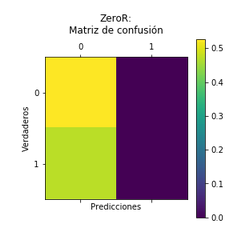
\includegraphics[width=57mm]{imagenes/hip_zeror}}
  \subfigure[SVM]{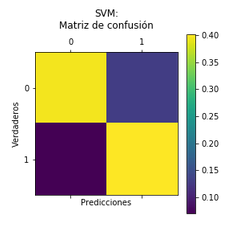
\includegraphics[width=57mm]{imagenes/hip_svm}}
  \subfigure[k-nn]{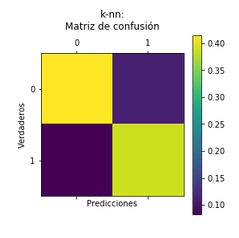
\includegraphics[width=57mm]{imagenes/hip_knn}}
\end{figure}

\begin{figure}[H]
  \centering
  \subfigure[Árbol de decisión]{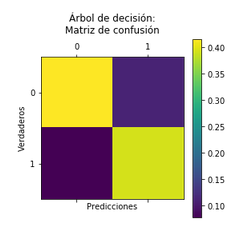
\includegraphics[width=58mm]{imagenes/hip_arbol}}
  \subfigure[MLP]{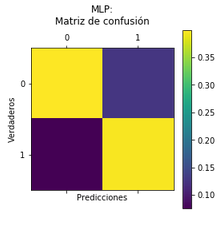
\includegraphics[width=55mm]{imagenes/hip_mlp}}
  \subfigure[Random Forest]{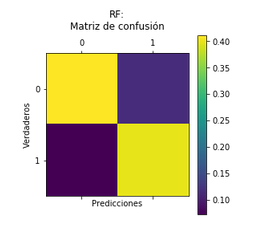
\includegraphics[width=60mm]{imagenes/hip_rf}}
\end{figure}

\vspace{-7mm}
Siempre interesa que estas matrices sean lo más parecido posible a una matriz diagonal. En nuestro caso es preferible que la fila inferior de la matriz sea más nítida que la de arriba, ya que esta corresponde a los tumores malignos y refleja cómo los clasificamos. 

Tenemos especial interés en que el número de pacientes con tumores malignos sin diagnosticar sean el mínimo posible. Como sabemos que las diferencias entre los distintos algoritmos son escasas, podemos considerar como medida de bondad el \texttt{FN}, que son exactamente estos pacientes con tumores malignos que han sido diagnosticados como benignos. Esta medida no hubiese sido buena usarla desde el principio, puesto que etiquetando a todos los pacientes como tumores malignos esta medida sería máxima pero no sería una solución factible a nuestro problema. Ahora que sabemos que el comportamiento de los modelos es muy similar y con el único propósito de discernir cuál de ellos ``resuelve'' mejor el problema, considero oportuno usarla.

El valor de la métrica \texttt{FN} en cada modelo viene representado en la casilla inferior izquierda de la matriz de confusión y es preferible que sea lo más bajo posible, es decir, que su color sea lo más azul oscuro posible. En la tabla mostrada al principio de la sección vemos que el modelo con menor \texttt{FN} es el SVM, que diagnostica un total de $64$ tumores como benignos siendo malignos. Estas instancias corresponden el $7.048\%$ de los datos. Como ya hemos comentado, el modelo SVM etiqueta más instancias como tumores malignos que el resto de modelos, y es por eso que es el modelo con mayor tasa de falsos positivos.

El siguiente modelo con menor número número de falsos negativos es el Random Forest, modelo que también poseía el mayor valor de \texttt{F1-Score}.

Los modelos con menor número de falsos negativos son el árbol de decisión y el k-nn. Son los que menos instancias clasifican como positivas, un total de $459$ y $454$ respectivamente.

Por consiguiente, para ``resolver'' el problema de clasificación de tumores yo usaría los modelos SVM y Random Forest.

Ya he ajustado varios parámetros del Random Forest en la sección de configuración de hiperparámetros consiguiendo mejorar su \texttt{F1-Score}, especialmente usando la poda Coste-Complejidad, por lo que considero que he intentado sacarle el mayor rendimiento posible al modelo usando el procesado de datos $3$. Si es verdad que este procesamiento no era el más prometedor para este modelo, por lo que una manera de mejorar el desempeño del modelo sería buscar un procesado de datos más propicio para él, ya sea el procesado $1$ o cualquier otro adaptado al modelo. Los árboles de decisión no necesitan normalizar los datos y pueden entrenar con valores perdidos, así que podría eliminarse alguno de estos pasos en el procesamiento.

Para mejorar los resultados del modelo SVM podríamos intentar utilizar un kernel no lineal.

\newpage
\section{Interpretación de resultados}

Uno de los modelos más interpretables es el árbol de decisión. Con el código:

\begin{lstlisting}
fig = plt.figure(figsize=(25,20))
_ = tree.plot_tree(tree_clf, 
                   feature_names=data.columns,  
                   class_names=["maligno","benigno"],
                   filled=True)

\end{lstlisting}

Podemos ver el árbol resultante al entrenar el modelo con el último conjunto de la validación cruzada. El modelo se entrena con $724$ instancias, dejando las $184$ restantes para validación.

\begin{figure}[H]
  \centering
  \subfigure[Árbol de decisión]{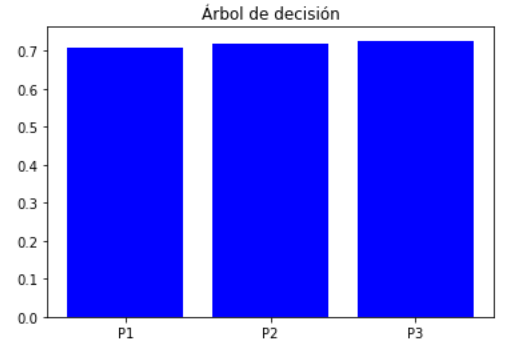
\includegraphics[width=180mm]{imagenes/arbol}}
\end{figure}

Primero resaltar que el árbol trabaja con valores normalizados. Para facilitar su lectura mostraremos la correspondencia en esta tabla:

\begin{center}
\begin{tabular}{|c|c|c|}
\hline
  \multicolumn{1}{|c|}{\textbf{Característica}}& \textbf{Sin normalizar} & \textbf{Normalizado} \\ \hline
  Shape  & 0 (I) & 0    \\ \hline
  Shape  & 1 (L) & 0.25 \\ \hline
  Shape  & 2 (N) & 0.5  \\ \hline
  Shape  & 3 (O) & 0.75 \\ \hline
  Shape  & 4 (R) & 1    \\ \hline
  Margen & 1     & 0    \\ \hline
  Margen & 2     & 0.25 \\ \hline
  Margen & 3     & 0.5  \\ \hline
  Margen & 4     & 0.75 \\ \hline
  Margen & 5     & 1    \\ \hline

\end{tabular}
\end{center}

En el caso de la edad, sabiendo que el valor mínimo que toma este atributo es 18 y el máximo 96, obtenemos que: $$\text{valor normalizado} = \frac{\text{valor real} - 18}{96 - 18} \Rightarrow \text{valor real} = 78(\text{valor normalizado}) + 18$$ Por tanto $0.532 \equiv 59.496$ años y $0.224 \equiv 35.472$ años. Una vez aclarado esto ya estamos en condiciones de interpretar el árbol.

Empezamos analizándo el nodo raíz. Como muestra la variable \texttt{samples}, el conjunto de entrenamiento está constituido por $724$ muestras, de las cuales $383$ son tumores benignos y $341$ son malignos. Esto último se refleja en \texttt{value}. Dado que hay más muestras benignas que malignas, la clase de ese nodo es ``benigno''. Esto implica que si el árbol terminase ahí, clasificaría todas las instancias como ``benignas'', es decir, se comportaría como el algoritmo \textit{ZeroR}. La variable \texttt{gini} es el valor de impureza del nodo.

La gráfica de la función del índice gini cuando hay dos clases es el corte entre la parábola azul y el plano magenta.

\begin{figure}[H]
  \centering
  \subfigure[Índice Gini]{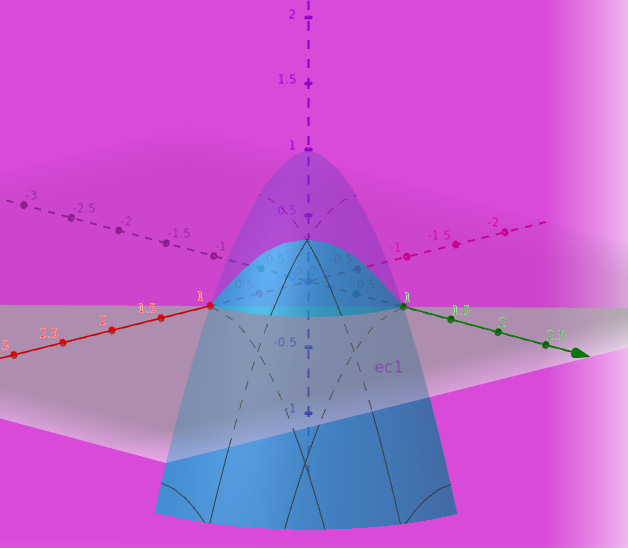
\includegraphics[width=70mm]{imagenes/graf_gini}}
\end{figure}

Como vemos, el índice vale $0$ cuando solo hay una de las dos clases en el nodo, no hay impureza. El índice alcanza su valor máximo, $0.5$, cuando las clases están balanceadas en el nodo.  En el nodo raíz, el valor del índice gini es $0.498$, es decir, las clases están casi balanceadas en un inicio, con lo cual la etiqueta asignada a ese nodo es poco representativa.\\
Finalmente, este nodo divide las muestras en según su márgen de masa. Si este margen es ``circunscribed'', es decir, si este atributo tiene valor $1$, le asigna la clase ``benigno''. En caso contrario sigue ramificando el árbol.

El nodo con las muestras con margen ``circunscribed'' es un nodo hoja. En él caen $281$ muestras del conjunto de entrenamiento, de las cuales $249$ corresponden a tumores  benignos y $32$ a malignos. Es por esto que la clase de este nodo es ``benigno''. El índice Gini de este nodo es $0.202$. Como hay impurezas en la hoja (muestras de ambas clases caen en esta hoja) es distinto de $0$, pero una clase es más frecuente que la otra. Como este árbol usa el criterio de poda coste-complejidad, a pesar de que caen elementos de ambas clases en la hoja no sigue desarrollándola.

El árbol se ramifica para clasificar las muestras con margen distinto de ``circunscribed''. Este conjunto está formado por $443$ muestras, de las cuales $134$ representan tumores benignos y $309$ malignos. Es por esto que al nodo se le asigna la clase ``maligno''. El índice Gini del nodo es $0.422$. En este nodo se ramifican las muestras entre aquellas con edad menor que $59.496$ años y mayor.

Nos centramos ahora en aquellas muestras cuyo atributo \textit{Age} es menor que $59.496$. Estas muestras vuelven a clasificarse en el siguiente nodo entre aquellas que tienen forma ``irregular'' y aquellas que no. Este nodo contiene $206$ instancias, de las cuales $93$ son tumores benignos y $113$ son malignos. La clase del nodo es por tanto ``maligno''. Los datos que caen en este nodo están casi balanceados, como muestra el índice Gini, que vale $0.495$.

Aquellos datos cuyo atributo \textit{Shape} tiene el valor ``irregular'' son otra vez clasificados entre aquellos con edad menor que $35.472$ años y aquellos con edad mayor. En este nodo de ramificación caen $140$ instancias, $46$ tumores benignos y $94$ malignos. Es por esto que la clase del nodo es ``maligno''. La variable \texttt{gini} del nodo vale $0.224$.

Hay $9$ datos cuyo atributo \textit{Shape} tiene el valor ``irregular'' y tienen menos de $35.472$ años. La clase del nodo es ``benigno'', debido a que $6$ de ellos corresponden a tumores benignos y los otros $3$ a malignos. El índice Gini del nodo es $0.444$, indicando que hay bastantes impurezas en la hoja. Debido al método de poda usado para evitar el sobreajuste del árbol, este nodo no vuelve a ramificarse, siendo por esto un nodo hoja.

Hay $131$ datos cuyo atributo \textit{Shape} tiene el valor ``irregular'' y tienen más de $35.472$ años. La clase del nodo es ``maligno'', debido a que $40$ de ellos corresponden a tumores benignos y los otros $91$ a malignos. El índice Gini del nodo es $0.424$, indicando que hay bastantes impurezas en la hoja. Debido al método de poda usado para evitar el sobreajuste del árbol, este nodo no vuelve a ramificarse, siendo por esto un nodo hoja.

Aquellos datos cuyo atributo \textit{Shape} no tiene el valor ``irregular'' son clasificados entre aquellos que tienen margen ``spiculated'' y los que no. En este nodo de ramificación caen $66$ instancias, $47$ tumores benignos y $19$ malignos. Es por esto que la clase del nodo es ``benigno''. La variable \texttt{gini} del nodo vale $0.41$.

Los datos con margen ``spiculated'' son $57$, $45$ son tumores benignos y el resto malignos. La clase del nodo pues es ``benigno''. Aunque este nodo no se ramifique, vemos que hay impurezas en él. Su índice Gini es $0.332$.

Los datos con margen distinto de ``spiculated'' son $9$, $2$ son tumores benignos y el resto malignos. La clase del nodo pues es ``maligno''. Aunque este nodo no se ramifique, vemos que hay impurezas en él. Su índice Gini es $0.346$.

Una vez que ya hemos analizado todos los datos con margen ``circunscribed'' y edad menor que $59.496$, analizamos el resto. Estos datos se ramifican también según su forma, entre aquellos con forma ``irregular'' o ``lobular'' y el resto. Este nodo de ramificación contiene $237$ instancias, $41$ corresponden a tumores benignos y $196$ a malignos, con lo que se le asigna la clase ``maligno'' a este nodo. La variable \texttt{gini} vale $0.286$.

Contamos con $202$ instancias con forma ``irregular'' o ``lobular'', $28$ representan tumores benignos y $174$ a malignos. El nodo con estas instancias es un nodo hoja, con indice Gini $0.239$. Las instancias en este nodo son clasificadas como tumores malignos.

Las $35$ muestras con otra forma son divididas según su margen, si este es ``ill-defined'' o ``spiculated'', o no lo es. El nodo de ramificación posee $13$ instancias correspondientes a tumores benignos y $22$ a malignos. Su clase es ``maligno''.

De las $35$ muestras, $26$ de ellas tienen margen ``ill-defined'' o ``spiculated''. La clase del nodo es ``maligno'', debido a que $5$ de ellas corresponden a tumores benignos y las otras $21$ a malignos. El índice Gini del nodo es $0.311$.

Las otras $9$ muestras se clasifican como tumores benignos, ya que en el nodo caen $8$ representando a tumores benignos y una a malignos. El índice Gini del nodo es $0.198$.

Como conclusión, el atrubuto más representativo es el márgen, ya que es aquel situado en la raíz del árbol. El $38.8\%$ de los datos de entrenamiento poseen margen ``circunscribed'', de los cuales el $88.61\%$ corresponden a tumores benignos. Por tanto, con esta división se clasifica el $34.39\%$ de los datos correctamente. Podríamos decir pues que esta característica es clave para la identificación de la severidad del tumor. Si es ``circunscribed'', lo más probable es que sea benigno. En caso contrario, podríamos clasificarlo como maligno. Esta división la vemos en las clases de los nodos de profundidad $1$. Notamos también que ninguna hoja está libre de impureza. Estas impurezas son el precio a pagar por evitar el sobreajuste del modelo.

Ejemplificamos el comportamiento del modelo con las siguientes instancias:

\begin{center}
\begin{tabular}{|c|c|c|c|c|c|}
\hline
  \multicolumn{1}{|c|}{\textbf{Dato}} & \textbf{BI-RADS} & \textbf{Age} & \textbf{Shape} & \textbf{Margin} & \textbf{Density}\\ \hline
  1 & 2  & 45 & R & 1 & 3 \\ \hline
  2 & 4  & 67 & L & 4 & 1 \\ \hline
\end{tabular}
\end{center}

\vspace{5mm}

Primero le aplicamos el preprocesado a ambas. Eliminamos la columna \textit{BI-RADS} y \textit{Density}:

\begin{center}
\begin{tabular}{|c|c|c|c|}
\hline
  \multicolumn{1}{|c|}{\textbf{Dato}} & \textbf{Age} & \textbf{Shape} & \textbf{Margin}\\ \hline
  1 & 20 & R & 1 \\ \hline
  2 & 67 & L & 4 \\ \hline
\end{tabular}
\end{center}

Normalizamos los datos:

\begin{center}
\begin{tabular}{|c|c|c|c|}
\hline
  \multicolumn{1}{|c|}{\textbf{Dato}} & \textbf{Age} & \textbf{Shape} & \textbf{Margin}\\ \hline
  1 & 0.0256 & 1    & 0    \\ \hline
  2 & 0.6282 & 0.25 & 0.75 \\ \hline
\end{tabular}
\end{center}

Veamos como clasifica el modelo los datos:

\begin{enumerate}
\item Su margen es menor que $0.125$, por tanto cae en la rama izquierda. Lo clasificamos como tumor benigno.
\item Su margen es mayor que $0.125$, por tanto cae en la rama derecha y seguimos recorriendo el árbol. Vemos que su edad es mayor que $0.532$, así que cae en la rama derecha de nuevo. Como su forma es menor que $0.375$, cae en la rama izquierda y clasificamos el tumor como maligno.
\end{enumerate}

 
\section{Contenido adicional}

Con el objetivo de tener una mejor percepción de los datos, implementé la función \texttt{dibuja\_gráfica} para visualizarlos.

\begin{lstlisting}
def dibuja_grafica(datos, target):
        fig = plt.figure()
        ax = fig.add_subplot(111, projection='3d')

        ax.set_xlabel('Age', fontsize = 10)
        ax.set_ylabel('Shape', fontsize = 10)
        ax.set_zlabel('Margin', fontsize = 10)

        azul_x = [] 
        azul_y = [] 
        azul_z = [] 
        
        rosa_x = [] 
        rosa_y = [] 
        rosa_z = [] 

        for i in range(0, len(datos)):
                if target.iloc[i] == 1:
                        azul_x.append(datos['Age'].iloc[i])
                        azul_y.append(datos['Shape'].iloc[i])
                        azul_z.append(datos['Margin'].iloc[i])
                else:
                        rosa_x.append(datos['Age'].iloc[i])
                        rosa_y.append(datos['Shape'].iloc[i])
                        rosa_z.append(datos['Margin'].iloc[i])

        ax.scatter(azul_x, azul_y, azul_z, c='c')
        ax.scatter(rosa_x, rosa_y, rosa_z, c='m')
        
        plt.show() 
      \end{lstlisting}

Tras aplicarle el porcesamiento $3$ a los datos, los visualizamos en $\mathbb{R}^3$, coloreando los correspondientes a tumores benignos de rosa y a los malignos de azul. El resultado es:

\begin{figure}[H]
  \centering
  \subfigure[ZeroR]{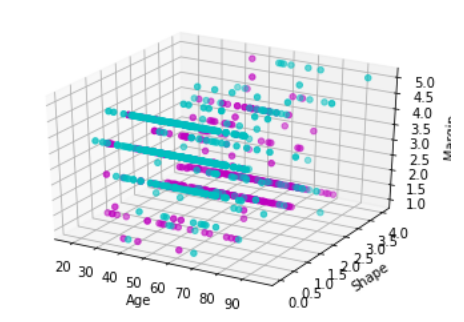
\includegraphics[width=100mm]{imagenes/datos}}
\end{figure}

Los datos no son separables por un hiperplano pero se concentran datos con la misma etiqueta en diversas regiones del espacio.

\section{Bibliografía}

\begin{itemize}
\item Dataset: \href{https://bigml.com/user/TotyB/gallery/dataset/509a98c6035d0706dd0001dd}{https://bigml.com/user/TotyB/gallery/dataset/509a98c6035d0706dd0001dd}
\item \label{Learning from Data} Yaser S, Abu-Mostafa, Malik Magdon-Ismail, Hsuan-Tien Lin, Learning from Data.
\item Tema 3: Modelos de predicción: Clasificación, regresión y series temporales.
\item Gini index y entropía: \\\href{https://www.bogotobogo.com/python/scikit-learn/scikt_machine\_learning\_Decision\_Tree\_Learning\_Informatioin\_Gain\_IG\_Impurity\_Entropy\_Gini\_Classification\_Error.php}{https://www.bogotobogo.com/python/scikit-learn/scikt\_machine\_learning\_Decision\_Tree\_Learning\_Informatioin\_Gain.php}
\item Cost-Complexity Pruning: \href{https://scikit-learn.org/stable/modules/tree.html\#minimal-cost-complexity-pruning}{https://scikit-learn.org/stable/modules/tree.html\#minimal-cost-complexity-pruning}
\item Early stopping: \href{https://machinelearningmastery.com/early-stopping-to-avoid-overtraining-neural-network-models/}{https://machinelearningmastery.com/early-stopping-to-avoid-overtraining-neural-network-models/}
\item Interpretación árbol de decisión: \href{https://towardsdatascience.com/scikit-learn-decision-trees-explained-803f3812290d}{https://towardsdatascience.com/scikit-learn-decision-trees-explained-803f3812290d}
\item Proyecto final de AA que hice con la colaboración de David Cabezas Berrido:\\ \href{https://github.com/dcabezas98/AA/tree/master/proyectoFinal}{https://github.com/dcabezas98/AA/tree/master/proyectoFinal}
\end{itemize}

\end{document}
